\documentclass[12pt]{report}
\usepackage{tikz}
\usepackage{parskip}
\usepackage{mathtools}
\usepackage{flexisym}



\begin{document}
\newcommand\tab[1][1cm]{\hspace*{#1}}

%title page
\author{Andre Gregoire}
\title{CIS770 Homework 3}
\maketitle

%problem 1
\textbf{ Problem1}\newline
\textit{1.1.}\newline
\begin{flushleft}
This DFA was built directly.  I first made a DFA to follow (abb*)* and then complemented it in order to fit the question.  I have a state $q_0$ that remembers if it has seen the first a, and a state another state $q_2$ that remember if there was any number of b's following the first a as well as a dead state, $q_1$ that is gone to if it does not fit the language requirements. There is also an initial state $q_\epsilon$, after this initial DFA was constructed I complemented it and the resulting DFA is below.
\end{flushleft}

\begin{center}
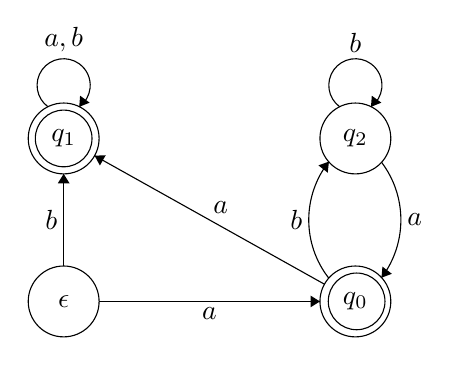
\begin{tikzpicture}[scale=0.15]
\tikzstyle{every node}+=[inner sep=0pt]
\draw [black] (11.3,-23.5) circle (3);
\draw (11.3,-23.5) node {$\epsilon$};
\draw [black] (36,-23.5) circle (3);
\draw (36,-23.5) node {$q_0$};
\draw [black] (11.3,-9.7) circle (3);
\draw [black] (38.8,-20.8,7) circle (2.4);
\draw (11.3,-9.7) node {$q_1$};
\draw [black] (11.3,-9.7) circle (2.4);
\draw [black] (36,-9.7) circle (3);
\draw (36,-9.7) node {$q_2$};
\draw [black] (14.3,-23.5) -- (33,-23.5);
\fill [black] (33,-23.5) -- (32.2,-23) -- (32.2,-24);
\draw (23.65,-24) node [below] {$a$};
\draw [black] (33.38,-22.04) -- (13.92,-11.16);
\fill [black] (13.92,-11.16) -- (14.37,-11.99) -- (14.86,-11.12);
\draw (24.59,-16.1) node [above] {$a$};
\draw [black] (9.977,-7.02) arc (234:-54:2.25);
\draw (11.3,-2.45) node [above] {$a,b$};
\fill [black] (12.62,-7.02) -- (13.5,-6.67) -- (12.69,-6.08);
\draw [black] (33.755,-21.536) arc (-141.91515:-218.08485:8.003);
\fill [black] (33.76,-11.66) -- (32.87,-11.98) -- (33.66,-12.6);
\draw (31.55,-16.6) node [left] {$b$};
\draw [black] (38.208,-11.706) arc (37.13588:-37.13588:8.106);
\fill [black] (38.21,-21.49) -- (39.09,-21.16) -- (38.29,-20.55);
\draw (40.35,-16.6) node [right] {$a$};
\draw [black] (34.677,-7.02) arc (234:-54:2.25);
\draw (36,-2.45) node [above] {$b$};
\fill [black] (37.32,-7.02) -- (38.2,-6.67) -- (37.39,-6.08);
\draw [black] (11.3,-20.5) -- (11.3,-12.7);
\fill [black] (11.3,-12.7) -- (10.8,-13.5) -- (11.8,-13.5);
\draw (10.8,-16.6) node [left] {$b$};
\end{tikzpicture}
\end{center}

\textit{1.2.}\newline

\textbf{Step 1.} Convert DFA to GNFA

\begin{center}
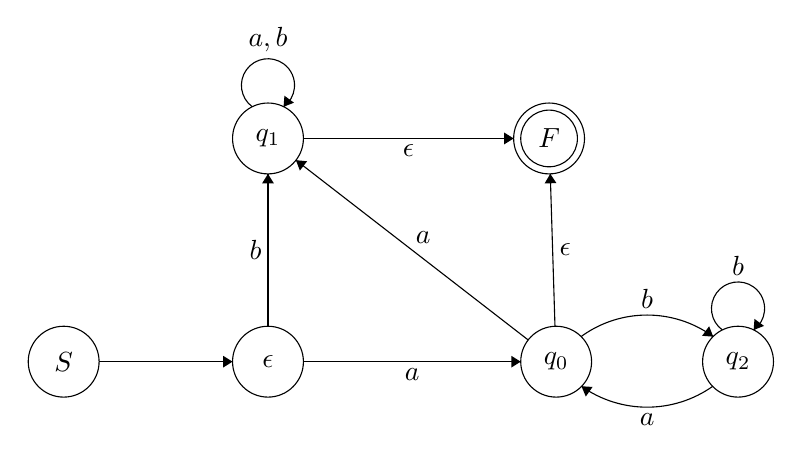
\begin{tikzpicture}[scale=0.15]
\tikzstyle{every node}+=[inner sep=0pt]
\draw [black] (27,-43.9) circle (3);
\draw (27,-43.9) node {$\epsilon$};
\draw [black] (51.4,-43.9) circle (3);
\draw (51.4,-43.9) node {$q_0$};
\draw [black] (27,-25) circle (3);
\draw (27,-25) node {$q_1$};
\draw [black] (66.8,-43.9) circle (3);
\draw (66.8,-43.9) node {$q_2$};
\draw [black] (9.7,-43.9) circle (3);
\draw (9.7,-43.9) node {$S$};
\draw [black] (50.8,-25) circle (3);
\draw (50.8,-25) node {$F$};
\draw [black] (50.8,-25) circle (2.4);
\draw [black] (30,-43.9) -- (48.4,-43.9);
\fill [black] (48.4,-43.9) -- (47.6,-43.4) -- (47.6,-44.4);
\draw (39.2,-44.4) node [below] {$a$};
\draw [black] (49.03,-42.06) -- (29.37,-26.84);
\fill [black] (29.37,-26.84) -- (29.7,-27.72) -- (30.31,-26.93);
\draw (40.15,-33.95) node [above] {$a$};
\draw [black] (25.677,-22.32) arc (234:-54:2.25);
\draw (27,-17.75) node [above] {$a,b$};
\fill [black] (28.32,-22.32) -- (29.2,-21.97) -- (28.39,-21.38);
\draw [black] (53.504,-41.779) arc (126.17151:53.82849:9.482);
\fill [black] (64.7,-41.78) -- (64.35,-40.9) -- (63.76,-41.71);
\draw (59.1,-39.45) node [above] {$b$};
\draw [black] (64.659,-45.984) arc (-54.71001:-125.28999:9.622);
\fill [black] (53.54,-45.98) -- (53.91,-46.85) -- (54.48,-46.04);
\draw (59.1,-48.25) node [below] {$a$};
\draw [black] (65.477,-41.22) arc (234:-54:2.25);
\draw (66.8,-36.65) node [above] {$b$};
\fill [black] (68.12,-41.22) -- (69,-40.87) -- (68.19,-40.28);
\draw [black] (27,-40.9) -- (27,-28);
\fill [black] (27,-28) -- (26.5,-28.8) -- (27.5,-28.8);
\draw (26.5,-34.45) node [left] {$b$};
\draw [black] (12.7,-43.9) -- (24,-43.9);
\fill [black] (24,-43.9) -- (23.2,-43.4) -- (23.2,-44.4);
\draw [black] (30,-25) -- (47.8,-25);
\fill [black] (47.8,-25) -- (47,-24.5) -- (47,-25.5);
\draw (38.9,-25.5) node [below] {$\epsilon$};
\draw [black] (51.3,-40.9) -- (50.9,-28);
\fill [black] (50.9,-28) -- (50.42,-28.81) -- (51.42,-28.78);
\draw (51.65,-34.44) node [right] {$\epsilon$};
\end{tikzpicture}
\end{center}

\pagebreak
\textbf{Step 2.} Remove $q_2$ and $q_1$

\begin{center}
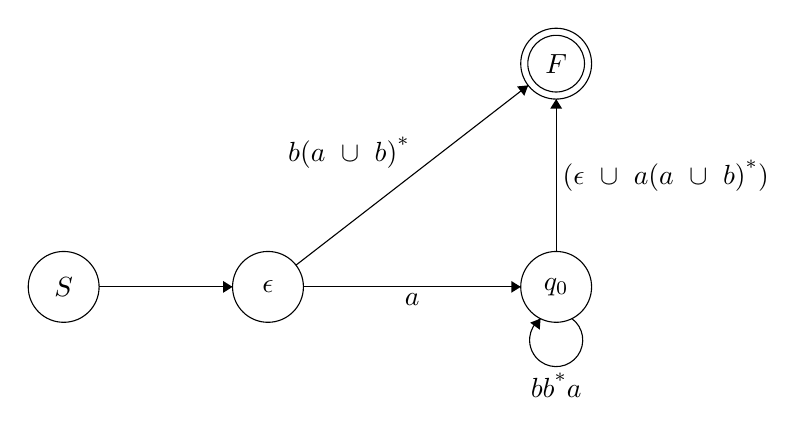
\begin{tikzpicture}[scale=0.15]
\tikzstyle{every node}+=[inner sep=0pt]
\draw [black] (27,-43.9) circle (3);
\draw (27,-43.9) node {$\epsilon$};
\draw [black] (51.4,-43.9) circle (3);
\draw (51.4,-43.9) node {$q_0$};
\draw [black] (9.7,-43.9) circle (3);
\draw (9.7,-43.9) node {$S$};
\draw [black] (51.4,-25) circle (3);
\draw (51.4,-25) node {$F$};
\draw [black] (51.4,-25) circle (2.4);
\draw [black] (30,-43.9) -- (48.4,-43.9);
\fill [black] (48.4,-43.9) -- (47.6,-43.4) -- (47.6,-44.4);
\draw (39.2,-44.4) node [below] {$a$};
\draw [black] (12.7,-43.9) -- (24,-43.9);
\fill [black] (24,-43.9) -- (23.2,-43.4) -- (23.2,-44.4);
\draw [black] (51.4,-40.9) -- (51.4,-28);
\fill [black] (51.4,-28) -- (50.9,-28.8) -- (51.9,-28.8);
\draw (51.9,-34.45) node [right] {$(\epsilon\mbox{ }\cup\mbox{ }a(a\mbox{ }\cup\mbox{ }b)\textsuperscript{*})$};
\draw [black] (52.723,-46.58) arc (54:-234:2.25);
\draw (51.4,-51.15) node [below] {$bb\textsuperscript{*}a$};
\fill [black] (50.08,-46.58) -- (49.2,-46.93) -- (50.01,-47.52);
\draw [black] (29.37,-42.06) -- (49.03,-26.84);
\fill [black] (49.03,-26.84) -- (48.09,-26.93) -- (48.7,-27.72);
\draw (33.86,-33.95) node [above] {$b(a\mbox{ }\cup\mbox{ }b)\textsuperscript{*}$};
\end{tikzpicture}
\end{center}

\textbf{Step 3.} Remove $q_0$ and $\epsilon$

\begin{center}
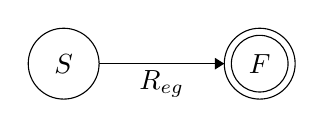
\begin{tikzpicture}[scale=0.15]
\tikzstyle{every node}+=[inner sep=0pt]
\draw [black] (9.7,-43.9) circle (3);
\draw (9.7,-43.9) node {$S$};
\draw [black] (26.3,-43.9) circle (3);
\draw (26.3,-43.9) node {$F$};
\draw [black] (26.3,-43.9) circle (2.4);
\draw [black] (12.7,-43.9) -- (23.3,-43.9);
\fill [black] (23.3,-43.9) -- (22.5,-43.4) -- (22.5,-44.4);
\draw (18,-44.4) node [below] {$R_{eg}$};
\end{tikzpicture}
\end{center}

Now that all the states have been removed we can put together the pieces to make $R_{eg}$ which is : \newline
\begin{equation*}
R_{eg} = b(a \cup b)\textsuperscript{*} \cup a(bb\textsuperscript{*}a)\textsuperscript{*}(\epsilon \cup a(a \cup b)\textsuperscript{*})
\end{equation*}

%problem 2
\textbf{Problem 2}\newline
\textit{2.1.} left(A) = $\{\epsilon$, 10$\}$

\textit{2.2.} left(A) = L(0\textsuperscript{*}1)

\textit{2.3.}
M = $(Q,\Sigma, \delta, q_0, F)$,  
M is the DFA that recognizes A, to determine if some word \textit{w} belongs to left(A) we can simultaneously check the forward path at the initial state and backward path at the final state of \textit{w} in our DFA M, the states of our new DFA are the same states as our old DFA M and the new initial state.

The new DFA M\textprime = $(Q\textprime, \Sigma, \delta\textprime, q_0\textprime, F\textprime)$ where: \newline
\tab Q\textprime = (Q x Q) $\cup$ $\{q_0\textprime\}$\newline
\tab F\textprime = $\{$(q,q) $\vert$ q $\in$ Q$\}$\newline
\tab $q_0\textprime$ =  $\{ q_0, F \}$ {\footnotesize: because we start at both ends of the original machine M}

\tab $\delta\textprime(q\textprime, a)$ = $\begin{cases}
	\{q_0\} \text{ x }F  							&\text{if } q\textprime  = q_0\textprime \text{ and }a = \epsilon\\
	\{(q_1\textprime, q_2\textprime) \vert \delta(q_1, a) = q_1\textprime and \delta(q_2, a) = q_2\textprime	&\text{if } q\textprime = (q_1, q_2) \text{ and } a \in \Sigma\\
	\emptyset 									& \text{else}\\
\end{cases}$



%problem 3
\textbf{Problem 3}
\begin{flushleft}
	Assume C is regular, for contradiction, with \textit{p} as the pumping lemma length.  let w = 1\textsuperscript{p}01\textsuperscript{p} and w $\in$ C. 
	
	\textit{x, y, z } such that \textit{w} = \textit{xyz} and has the following properties:\newline
	\tab $\vert\textit{y}\vert$ $>$ 0\newline
	\tab $\vert\textit{xy}\vert$ $\leq$ \textit{p}
	
	Assume \textit{x} = 1\textsuperscript{i}, \textit{y} = 1\textsuperscript{j}, \textit{z} = 1\textsuperscript{k}01\textsuperscript{p}, where \textit{i+j+k} = \textit{p} and j $>$ 0.
	
	Now \textit{w}\textprime = \textit{xy\textsuperscript{0}z} = 1\textsuperscript{i+k}01\textsuperscript{p}. The number of ones preceding the first 0 is less than \textit{p} and there are \textit{p} ones following the first zero.  Because there are \textit{p}-1 number of ones preceding the first zero there must be \textit{p}-1 number of ones following the first zero however there are \textit{p} number of ones following so \newline \textit{w} $\notin$ C.  C does not satisfy the pumping lemma and therefore is not regular.
	
\end{flushleft}


%problem 4
\textbf{Problem 4}\newline
\textit{4.1.}
\begin{flushleft}
	A = $F \cap L(ab\textsuperscript{*}c\textsuperscript{*})$ = $\{ab\textsuperscript{n}c\textsuperscript{n} \vert n \geq 0\}$, we can define a homomorphism h:$\{\textit{a,b,c}\}\textsuperscript{*} \rightarrow \{0,1\}\textsuperscript{*}$ where h(a) = $\epsilon$, h(b) = 0 and h(c) = 1.  Now if we apply the homomorphism to our language A, h(A) = $\{0\textsuperscript{n}1\textsuperscript{n} \vert n \geq 0\} = L_{0\textsuperscript{n}1\textsuperscript{n}}$\newline
	
	Now consider h(A) to be regular, and let p be the pumping length for $L_{0\textsuperscript{n}1\textsuperscript{n}}$.\newline
	\textit{w} = 0\textsuperscript{p}1\textsuperscript{p}\newline
	Since $\vert \textit{w} \vert \textgreater  p$ there are \textit{x, y, z} such that \textit{w} = \textit{xyz} where:\newline
	\tab $\vert xy \vert \leq p$ \newline
	\tab $\vert y \vert \textgreater 0$\newline
	\tab and  x = 0\textsuperscript{r}, y = 0\textsuperscript{s}, z = 0\textsuperscript{t}1\textsuperscript{p} where $\vert y \vert$ \textgreater 0 and s \textgreater 0
	\begin{equation*}
		xy\textsuperscript{0}z = 0\textsuperscript{r}\epsilon0\textsuperscript{t}1\textsuperscript{p} = 0\textsuperscript{r+t}1\textsuperscript{p}
	\end{equation*}
	since \textit{r+t} \textless \textit{ p}, xy\textsuperscript{0}z $\notin$ $L_{0\textsuperscript{n}1\textsuperscript{n}}$ this contradicts that h(A) is regular, thus proving F is also not regular.
\end{flushleft}
	
\pagebreak
\textit{4.2.}
\begin{flushleft}

Let \textit{p} = 3, where any \textit{w} $\in$ F where $\vert w \vert$  $\geq$ p.\newline
Since \textit{i} cannot be 0 and the word \textit{w} is already divided for the case \textit{i} = 1, we only need to show for cases when \textit{i} = 2 and when \textit{i} $\neq$ 2, or when it is greater than 2.

If \textit{i} = 2, divide w into \textit{x,y,z}.  \textit{x} = aa, \textit{y} can be the next symbol and \textit{z} makes up what is left of word \textit{w}.  This satifies the properties that $\vert xy \vert$ $\leq$ p, and  \newline $\vert y \vert$ $>$ 0.

If \textit{i} $\neq$ 2, divide w into \textit{x,y,z}. ...

\textbf{Note:} come back and finish  4.2

\end{flushleft}

\end{document}
